\documentclass[tikz]{standalone}
\begin{document}
	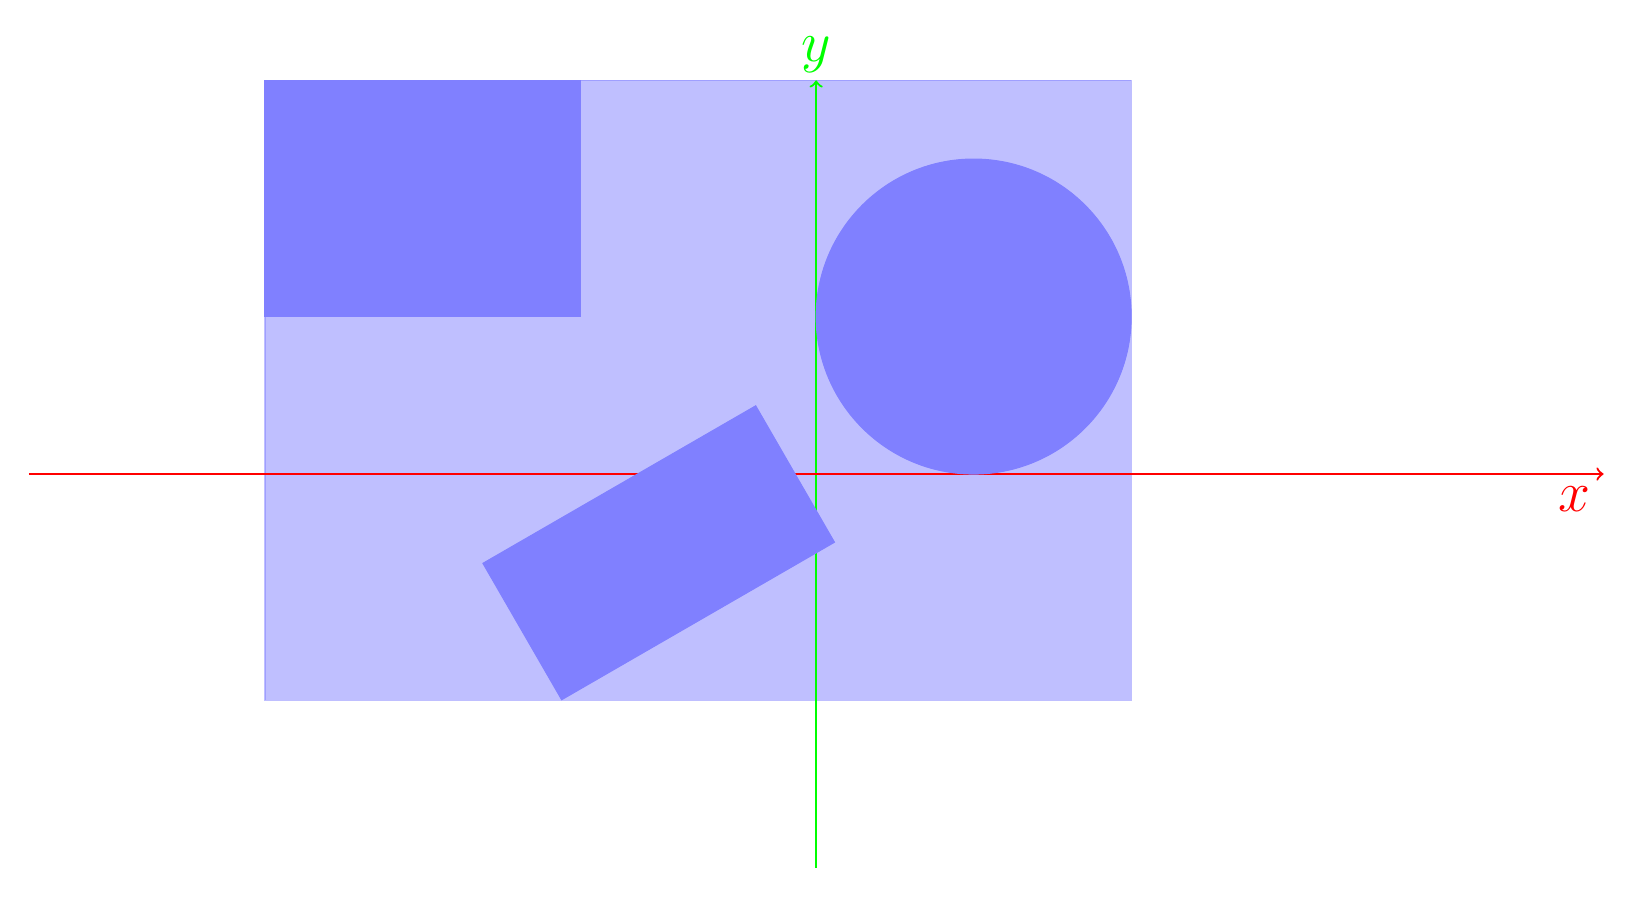
\begin{tikzpicture}
		
		\filldraw [blue!50, semitransparent] (-7, -2.875) rectangle (4,5);
		
		\draw[green,thick, ->] (0,-5) -- (0,5) node[above=-1]{\huge $y$};
		\draw[red,thick, ->] (-10,0) -- (10,0) node[below left=1]{\huge $x$};
		
		\filldraw[blue!50, rotate around={30:(-2,-1)}] (0,0) rectangle (-4,-2);
		\filldraw[blue!50] (2,2) circle (2);
		\filldraw[blue!50] (-3,2) rectangle (-7,5);
		
	\end{tikzpicture}
\end{document}